\chapter{Theoretische Grundlagen}

Um die Funktionsweise von Augmented Reality (AR) und verwandten Technologien zu verstehen, ist ein grundlegendes Wissen über die zugrunde liegenden Konzepte und Techniken erforderlich. In diesem Kapitel werden die theoretischen Grundlagen der Computer Vision und Computergrafik erläutert, die für die Entwicklung von AR-Anwendungen relevant sind. Dabei wird vor der Fokus vor allem auf die Konzepte gelegt, die eine Relevanz für mobile AR-Anwendungen haben. Dazu gehören die Rekonstruktion von 3D-Szenen, die Kamerakalibrierung, die Sensorik, das Tracking und Rendering von virtuellen Objekten. (\cite{doerner2022virtual})

\section{Dreidimensionale Computergrafik}

In der Computergrafik werden dreidimensionale Objekte, auch als Modelle bezeichnet, durch geometrische und relationale Informationen beschrieben. Diese Objekte bestehen in der Regel aus Polygonen, die durch ihre Eckpunkte (Vertices) definiert sind. Ein Polygon ist eine geschlossene Fläche, die durch das Verbinden der Vertices mit geraden Linien entsteht. Ein 3D-Modell wird in einem kartesischen Koordinatensystem beschrieben, wobei die Positionen der Vertices durch ihre \(x\)-, \(y\)- und \(z\)-Koordinaten angegeben werden. (\cite{kore2018space})

Das einfachste Polygon ist ein Dreieck, das nur drei Eckpunkte benötigt. Dreiecke sind planar und konvex, was sie ideal für Berechnungen in der Computergrafik macht, wie beispielsweise bei der Beleuchtung oder Kollisionserkennung. Obwohl komplexere Polygone existieren, werden diese oft in Dreiecke zerlegt, da sie von Grafikpipelines effizienter verarbeitet werden können. Solche Modelle bestehen dann aus Dreiecksnetzen (Meshes), die als Arrays von Vertices und Indizes gespeichert werden. (\cite{wikipedia2023polygons})

Virtuelle 3D-Szenen und Objekte werden in einem kartesischen Koordinatensystem beschrieben. Dieses Koordinatensystem wird üblicherweise als Weltkoordinatensystem bezeichnet, in dem die \(x\)-, \(y\)- und \(z\)-Achsen die drei Dimensionen repräsentieren. In einem rechtshändigen Koordinatensystem zeigt die \(x\)-Achse nach rechts, die \(y\)-Achse nach oben und die \(z\)-Achse nach vorne. Die Position eines Objekts im Raum wird oft mithilfe einer Transformationsmatrix beschrieben. (\cite{appledevdoc, usau2023appleARCamera})

\section{Matrixalgebra}

Das Anwenden von mathematischen Operationen auf Matrizen ist ein grundlegendes Konzept für viele Algorithmen in der Computer Vision. Diese Arbeit setzt voraus, dass der Leser mit den Grundladen der Matrixalgebra vertraut ist. Im Folgenden werden dennoch die wichtigsten Operationen und Konzepte anhand der Transformationen in der Computergrafik erläutert.

Unter der Transformation eines Objektes in einer 3D-Szene versteht man das Verschieben, Drehen oder Skalieren dieses Objektes. Diese Vorgänge können durch Transformationsmatrizen beschrieben werden, die einheitlich auf alle Vertices eines Objekts angewendet werden. Solche Matrizen haben typischerweise die Größe \(4 \times 4\) und kombinieren Translation, Rotation und Skalierung. Dies hat den Vorteil, dass alle Transformationen in einer einzigen Matrix zusammengefasst werden können, was die Berechnungen effizienter macht. (\cite{jazz2020transformMatrix, pezzi2021matrices, freescale2010math3d})

\subsection{Translation}

Die Translation verschiebt ein Objekt entlang der \(x\)-, \(y\)- oder \(z\)-Achse. Die Transformationsmatrix für eine Translation ist wie folgt definiert:

\begin{equation}
\begin{bmatrix}
x' \\ y' \\ z' \\ 1
\end{bmatrix}
=
\begin{bmatrix}
1 & 0 & 0 & t_x \\
0 & 1 & 0 & t_y \\
0 & 0 & 1 & t_z \\
0 & 0 & 0 & 1
\end{bmatrix}
\begin{bmatrix}
x \\ y \\ z \\ 1
\end{bmatrix}
\end{equation}

Hierbei verschieben die Parameter \(t_x\), \(t_y\) und \(t_z\) das Objekt entlang der jeweiligen Achsen.

\subsection{Rotation}

Die Rotation eines Objekts erfolgt um eine der drei Achsen. Die Rotationsmatrizen sind für jede Achse wie folgt definiert:

\paragraph{Rotation um die \(x\)-Achse:}
\begin{equation}
\begin{bmatrix}
1 & 0 & 0 & 0 \\
0 & \cos(\alpha) & -\sin(\alpha) & 0 \\
0 & \sin(\alpha) & \cos(\alpha) & 0 \\
0 & 0 & 0 & 1
\end{bmatrix}
\end{equation}

\paragraph{Rotation um die \(y\)-Achse:}
\begin{equation}
\begin{bmatrix}
\cos(\alpha) & 0 & \sin(\alpha) & 0 \\
0 & 1 & 0 & 0 \\
-\sin(\alpha) & 0 & \cos(\alpha) & 0 \\
0 & 0 & 0 & 1
\end{bmatrix}
\end{equation}

\paragraph{Rotation um die \(z\)-Achse:}
\begin{equation}
\begin{bmatrix}
\cos(\alpha) & -\sin(\alpha) & 0 & 0 \\
\sin(\alpha) & \cos(\alpha) & 0 & 0 \\
0 & 0 & 1 & 0 \\
0 & 0 & 0 & 1
\end{bmatrix}
\end{equation}

Die Reihenfolge, in der Rotationen um verschiedene Achsen durchgeführt werden, ist entscheidend, da sie die finale Orientierung und Position des Objektes beeinflussen. Diese Reihenfolge wird durch Euler-Winkel beschrieben.

\subsection{Skalierung}

Die Skalierung verändert die Größe eines Objekts proportional entlang der \(x\)-, \(y\)- und \(z\)-Achsen. Die Skalierungsmatrix ist wie folgt definiert:

\begin{equation}
\begin{bmatrix}
x' \\ y' \\ z' \\ 1
\end{bmatrix}
=
\begin{bmatrix}
s_x & 0 & 0 & 0 \\
0 & s_y & 0 & 0 \\
0 & 0 & s_z & 0 \\
0 & 0 & 0 & 1
\end{bmatrix}
\begin{bmatrix}
x \\ y \\ z \\ 1
\end{bmatrix}
\end{equation}

Hierbei sind \(s_x\), \(s_y\) und \(s_z\) die Skalierungsfaktoren entlang der jeweiligen Achsen.

\subsection{Anwendung der Transformationen}

Die lokalen Koordinaten eines Objekts können mithilfe einer Transformationsmatrix in Weltkoordinaten umgerechnet werden:

\begin{equation}
P_{world} = T_{object} \cdot P_{object}
\end{equation}

Hierbei ist \(T_{object}\) die Transformationsmatrix des Objekts, und \(P_{object}\) sind die lokalen Koordinaten. Das Ergebnis \(P_{world}\) beschreibt die Position des Objekts im Weltkoordinatensystem.

\section{Kalibrierung}

In Augmented-Reality-Anwendungen ist eine präzise Überlagerung digitaler Informationen auf die reale Welt essenziell, um ein realistisches und funktionales Benutzererlebnis zu schaffen. Die Kamerakalibrierung spielt hierbei eine entscheidende Rolle, da sie sicherstellt, dass virtuelle Objekte korrekt positioniert, skaliert und perspektivisch angepasst in die physische Umgebung integriert werden.

Die Kalibrierung umfasst die Bestimmung der intrinsischen Parameter der Kamera. Diese beschreiben die optischen Eigenschaften der Kamera, wie Brennweiten, Verzerrungen und die Position des optischen Zentrums. Das Ziel ist es, mithilfe dieser Paramater die extrinsischen Parameter der Kamera zu berechnen, die die Position und Orientierung der Kamera im Raum festlegen. Dadurch wird die Transformation von zweidimensionalen Bildpunkten in dreidimensionale Weltkoordinaten ermöglicht.

\begin{figure}
    \centering
    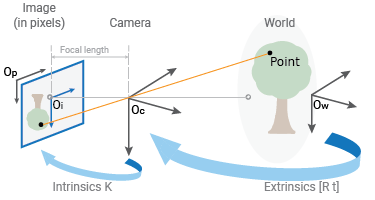
\includegraphics[ width=.5\textwidth ]{calibration-cameramodel-coords}
    \caption{Modell für die Kamerakalibrierung\label{fig:Kalibrierung}}\par
\end{figure}

Mathematisch wird die Transformation durch die Gleichung \( x = PX \) beschrieben, wobei:

\begin{itemize}
    \item \( x \) die Bildkoordinaten in Pixeln sind,
    \item \( P \) die Projektionsmatrix ist und
    \item \( X \) die Weltkoordinaten eines Objekts darstellt.
\end{itemize}

Die Projektionsmatrix \( P \) setzt sich aus der intrinsischen Matrix \( K \) sowie der Rotationsmatrix \( R \) und dem Translationsvektor \( t \) zusammen:
\[
P = K[R|t]
\]

Die intrinsische Matrix \( K \) wird folgendermaßen definiert:
\[
K = 
\begin{bmatrix}
f_x & s & c_x \\
0 & f_y & c_y \\
0 & 0 & 1
\end{bmatrix}
\]
\begin{itemize}
    \item \( f_x \) und \( f_y \): Brennweiten der Kamera in Pixeln, bezogen auf die horizontalen und vertikalen Achsen.
    \item \( c_x \) und \( c_y \): Koordinaten des optischen Zentrums in Pixeln.
    \item \( s \): Skew-Faktor, der berücksichtigt, ob die Kameraachsen orthogonal sind.
\end{itemize}

Um die Lens-Distortion zu korrigieren, werden oft Polynommodelle, wie das Brown-Conrady-Modell, verwendet. Dieses Modell beschreibt die radiale und tangentialen Verzerrungen der Linse und wird durch die Koeffizienten \( k_1, k_2, k_3 \) und \( p_1, p_2 \) definiert.

Moderne AR-Plattformen wie ARKit oder ARCore integrieren den Kalibrierungsprozess automatisch. ARKit speichert intrinsische Parameter in der Klasse \texttt{AVCameraCalibrationData} und berechnet die extrinsischen Parameter durch die Inertial Measurement Unit (IMU) des Geräts, welche Positions- und Orientierungsdaten liefert.

\section{Sensorik}

Die Erfassung der Umgebung in Augmented-Reality-Anwendungen erfolgt mithilfe verschiedener Sensoren, die Daten über die physische Welt liefern. Je nach Anwendungsfall und Eingabegerät können unterschiedliche Sensoren verwendet werden, um die Position und Bewegung des Geräts zu bestimmen. Zu den wichtigsten Sensoren für mobile AR-Anwendungen gehören:

\begin{itemize}
    \item \textbf{Kamera}: Die Kamera liefert visuelle Informationen über die Umgebung und wird zur Erkennung von Markern, Features oder Objekten verwendet.
    \item \textbf{LiDAR}: LiDAR (Light Detection and Ranging) ist ein Sensor, der die Entfernung zu Objekten mithilfe eines Lasers misst.
    \item \textbf{Gyroskop}: Das Gyroskop misst die Winkelgeschwindigkeit des Geräts und wird zur Erfassung von Drehbewegungen verwendet.
    \item \textbf{Beschleunigungsmesser}: Der Beschleunigungsmesser misst die Beschleunigung des Geräts und wird zur Erfassung von linearen Bewegungen verwendet.
    \item \textbf{Magnetometer}: Das Magnetometer misst das Magnetfeld des Geräts und wird zur Bestimmung der Ausrichtung im Raum verwendet.
    \item \textbf{GPS}: Das GPS (Global Positioning System) bestimmt die geografische Position des Geräts und wird zur Navigation und Lokalisierung verwendet.
\end{itemize}

Sensoren wie Gyroskop, Beschleunigungsmesser und Magnetometer werden oft in einem sogenannten IMU (Inertial Measurement Unit) kombiniert, um die Bewegung des Geräts in sechs Freiheitsgraden (3D-Position und -Orientierung) zu erfassen. 

Bei vielen Tracking-Verfahren werden eine Kombination von Sensoren verwendet, um die Genauigkeit und Zuverlässigkeit der Positionsschätzung zu verbessern. Beispielsweise kann die Kamera für visuelle Tracking-Anwendungen verwendet werden, während das IMU für die Schätzung der Bewegung des Geräts verwendet wird. Durch die Fusion von Daten aus verschiedenen Sensoren können AR-Anwendungen eine präzise und konsistente Darstellung der virtuellen Objekte in der realen Welt erreichen.

\section{Structure from Motion}

Structure from Motion (SfM) ist eine Technik aus der Computer Vision, die verwendet wird, um die 3D-Struktur einer Szene aus einer Reihe von 2D-Bildern zu rekonstruieren. SfM basiert auf der Triangulation von Punkten, die in verschiedenen Bildern sichtbar sind, um die Positionen der Sensoren und der Punkte in der Szene zu bestimmen.

Da SfM die Grundlage vieler AR-Verfahren darstellt und in verbesserter bzw. abgewandelter Form in vielen AR-Frameworks (z.B. SLAM, siehe Kapitel 4.7) eingesetzt wird, ist es wichtig, die grundlegenden Schritte und Algorithmen zu verstehen, die bei der Rekonstruktion von 3D-Szenen verwendet werden. Diese werden im Folgenden erläutert.

\subsection{Feature Detection und Matching}

Bei der Feature Detection bzw. beim Feature Maching werden Merkmale in verschiedenen Bildern identifiziert und korrespondierende Merkmale gefunden. Dieser Schritt ist entscheidend, um die Bewegung der Kamera (Tracking) und die 3D-Struktur der Szene zu bestimmen. Es gibt verschiedene Algorithmen, die für das Erkennen und Nachverfolgen von Feature-Punkten verwendet werden können, wie z. B. SIFT (Scale-Invariant Feature Transform), SURF (Speeded-Up Robust Features) oder ORB (Oriented FAST and Rotated BRIEF). Diese Algorithmen setzen sich grundsätzlich aus drei Teilen zusammen:

\begin{enumerate}
    \item Feature Detector oder Keypoint Detector
    \item Feature Descriptor
    \item Feature Matching Algorithm
\end{enumerate}

Der Feature Detector identifiziert charakteristische Punkte im Bild, die sich durch hohe Kontraste oder markante Strukturen auszeichnen. Diese Punkte, auch als Keypoints bezeichnet, dienen als Referenz für spätere Berechnungen. Anschließend erstellt der Feature Descriptor eine numerische Beschreibung für jedes erkannte Merkmal, um sie über mehrere Bilder hinweg vergleichbar zu machen. Diese Deskriptoren bestehen in der Regel aus Vektoren, die die Helligkeitsverteilung um den jeweiligen Feature-Punkt erfassen. Schließlich vergleicht der Feature Matching Algorithmus die Deskriptoren aus verschiedenen Bildern, um korrespondierende Merkmale zu finden, die wiederum zur Schätzung der Kamerabewegung genutzt werden.

Ein besonders effizienter und robuster Algorithmus ist ORB, der auf den Methoden FAST (Features from Accelerated Segment Test) und BRIEF (Binary Robust Independent Elementary Features) basiert. Der FAST-Algorithmus erkennt Punkte mit starken Helligkeitsänderungen, indem er benachbarte Pixel in einem Kreis um den zu prüfenden Pixel vergleicht. Übersteigt die Anzahl der signifikant helleren oder dunkleren Pixel einen bestimmten Schwellenwert, wird der Punkt als Feature identifiziert. Anschließend berechnet BRIEF für jedes erkannte Feature binäre Deskriptoren, indem zufällig gewählte Pixelpaare innerhalb der Umgebung des Feature-Punkts verglichen werden. Die resultierenden binären Deskriptoren sind besonders effizient in der Berechnung und Speicherung. Um die erkannten Merkmale schnell und zuverlässig zuzuordnen, kommt die Fast Library for Approximate Nearest Neighbors (FLANN) zum Einsatz, die eine leistungsstarke Methode zur Suche nach korrespondierenden Features bietet.

Neben klassischen Verfahren wie ORB gewinnen Deep-Learning-Modelle zunehmend an Bedeutung für das Feature Matching. Besonders Convolutional Neural Networks (CNNs) und Transformer-Modelle liefern vielversprechende Ergebnisse. Ein Beispiel hierfür ist XFeat (Accelerated Features), ein optimiertes neuronales Netzwerk, das die Merkmalsextraktion beschleunigt. Auch OmniGlue, eine Kombination aus CNNs und Transformer-Modellen, setzt neue Maßstäbe in der robusten und anpassungsfähigen Feature-Matching-Strategie. Diese modernen Ansätze bieten oft eine höhere Genauigkeit und Stabilität, insbesondere in komplexen Szenen oder bei stark variierenden Lichtverhältnissen.

\subsection{Camera Pose Estimation}

Die Schätzung der Kameraposition ist ein essenzieller Schritt in der SfM-Pipeline, da sie die Position und Orientierung der Kamera in jedem Bild bestimmt. Diese Informationen sind entscheidend für die Rekonstruktion der 3D-Struktur der Szene und die Bestimmung der extrinsischen Kameraparameter.

Geht man davon aus, dass die intrinsischen Parameter der Kamera bekannt sind und mehrere Bilder mit korrespondierenden Punkten vorliegen, kann die Kameraposition mithilfe der Essential Matrix \(E\) berechnet werden. Diese Matrix beschreibt die geometrische Beziehung zwischen zwei Bildern und ermöglicht die Bestimmung von Rotation und Translation der Kamera. Die grundlegende Bedingung für die Berechnung der extrinsischen Parameter lautet:

\begin{equation}
x'^T E x = 0
\end{equation}

Diese Gleichung beschreibt die Epipolargeometrie, wobei \( x \) und \( x' \) die korrespondierenden Punkte in den beiden Bildern darstellen. Die Essential Matrix kann durch den Five-Point-Algorithmus geschätzt werden, der im kalibrierten Fall mindestens fünf korrespondierende Punkte benötigt, um eine eindeutige Lösung zu liefern.

Sobald die Essential Matrix bestimmt wurde, kann sie mithilfe der Singulärwertzerlegung (SVD) in die Rotationsmatrix \( R \) und die Translationsmatrix \( t \) der Kamera zerlegt werden:

\begin{equation}
E = R [t]_x
\end{equation}

Diese Zerlegung erlaubt es, die Bewegung der Kamera zwischen den Bildern präzise zu bestimmen.

\subsection{Dreidimensionale Rekonstruktion}

Die dreidimensionale Rekonstruktion einer Szene überführt die zweidimensionalen Bilddaten einer Kamera in ein 3D-Modell. Dabei werden sowohl die Kameraparameter als auch die Translation und Rotation der Kamera sowie die korrespondierenden Feature-Punkte aus dem Feature Matching verwendet, um die Positionen der Punkte im Raum zu berechnen und so eine präzise 3D-Darstellung der Szene zu erstellen.

Ein zentraler Schritt in der 3D-Rekonstruktion ist die Triangulation, bei der die kartesischen Koordinaten eines Feature-Punktes im Weltkoordinatensystem ermittelt werden. Ein einfaches Verfahren zur Bestimmung dieser Koordinaten besteht darin, den 3D-Strahlen zu folgen, die von den Kamerazentren \( c_j \) in die Richtungen \( \hat{v_j} \) verlaufen. Der gesuchte Punkt \( p_0 \) ist derjenige, der sich im minimalen Abstand zu allen Strahlen befindet. Die Richtungen \( \hat{v_j} \) werden durch die Transformation der 2D-Bildpunkte mittels der Kameramatrizen beschrieben. Der Punkt \( p_0 \) wird dabei durch Minimierung der quadratischen Abstände zwischen den Strahlen und dem Punkt berechnet.

\begin{figure}
    \centering
    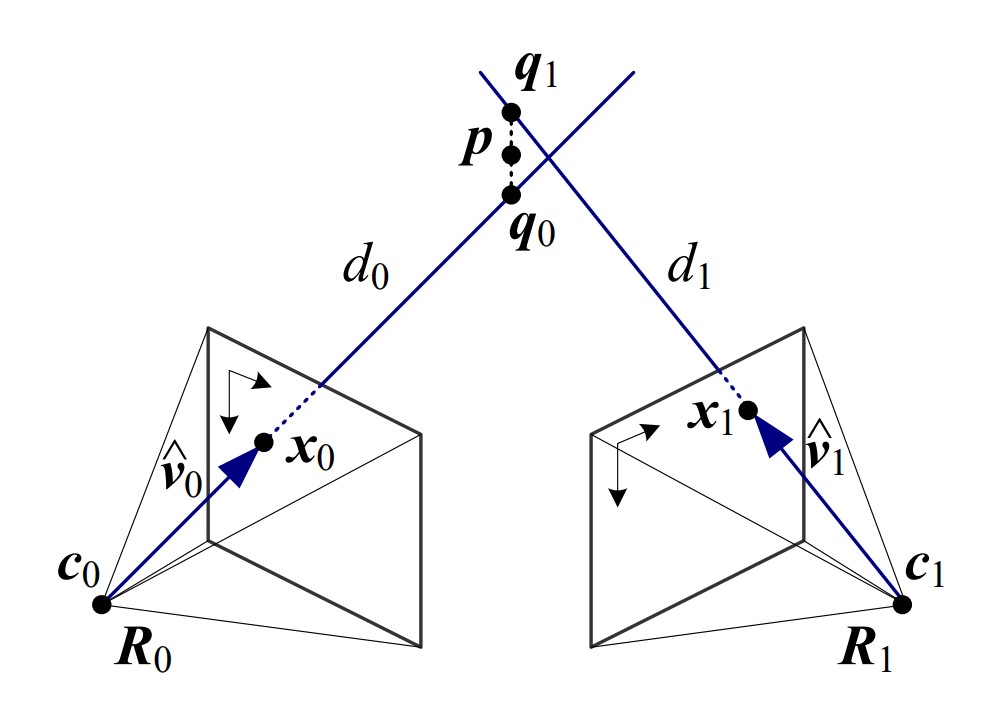
\includegraphics[width=.5\textwidth]{Triangulation}
    \caption{Dreidimensionale Triangulation mit zwei Bildern\label{fig:Triangulation}}\par
\end{figure}

Abbildung \ref{fig:Triangulation} zeigt die grafische Darstellung der Triangulation eines Punktes im dreidimensionalen Raum. Mathematisch wird dieser Prozess durch die folgende Gleichung beschrieben:

\[
p = \left( \sum_j \left( I - \hat{v_j} \hat{v_j}^T \right) \right)^{-1} \left( \sum_j \left( I - \hat{v_j} \hat{v_j}^T \right) c_j \right)
\]

Das Ergebnis der Triangulation ist eine sogenannte Punktwolke (Point Cloud), die die 3D-Struktur der Szene abbildet. Diese Punktwolke kann anschließend weiterverarbeitet werden, um ein detailliertes 3D-Modell der Szene zu erstellen. Ein wichtiger Schritt in dieser Weiterverarbeitung ist die Oberflächenrekonstruktion (Plane Detection), bei der die Punktwolke in Flächen unterteilt wird, um die Oberflächen von Objekten im Raum zu bestimmen. Zur Durchführung der Oberflächenrekonstruktion wird häufig der RANSAC-Algorithmus (Random Sample Consensus) eingesetzt. Dieser Algorithmus erkennt Ausreißer in den Daten und schätzt die Flächen anhand der verbleibenden, konsistenten Punkte.

\begin{figure}
    \centering
    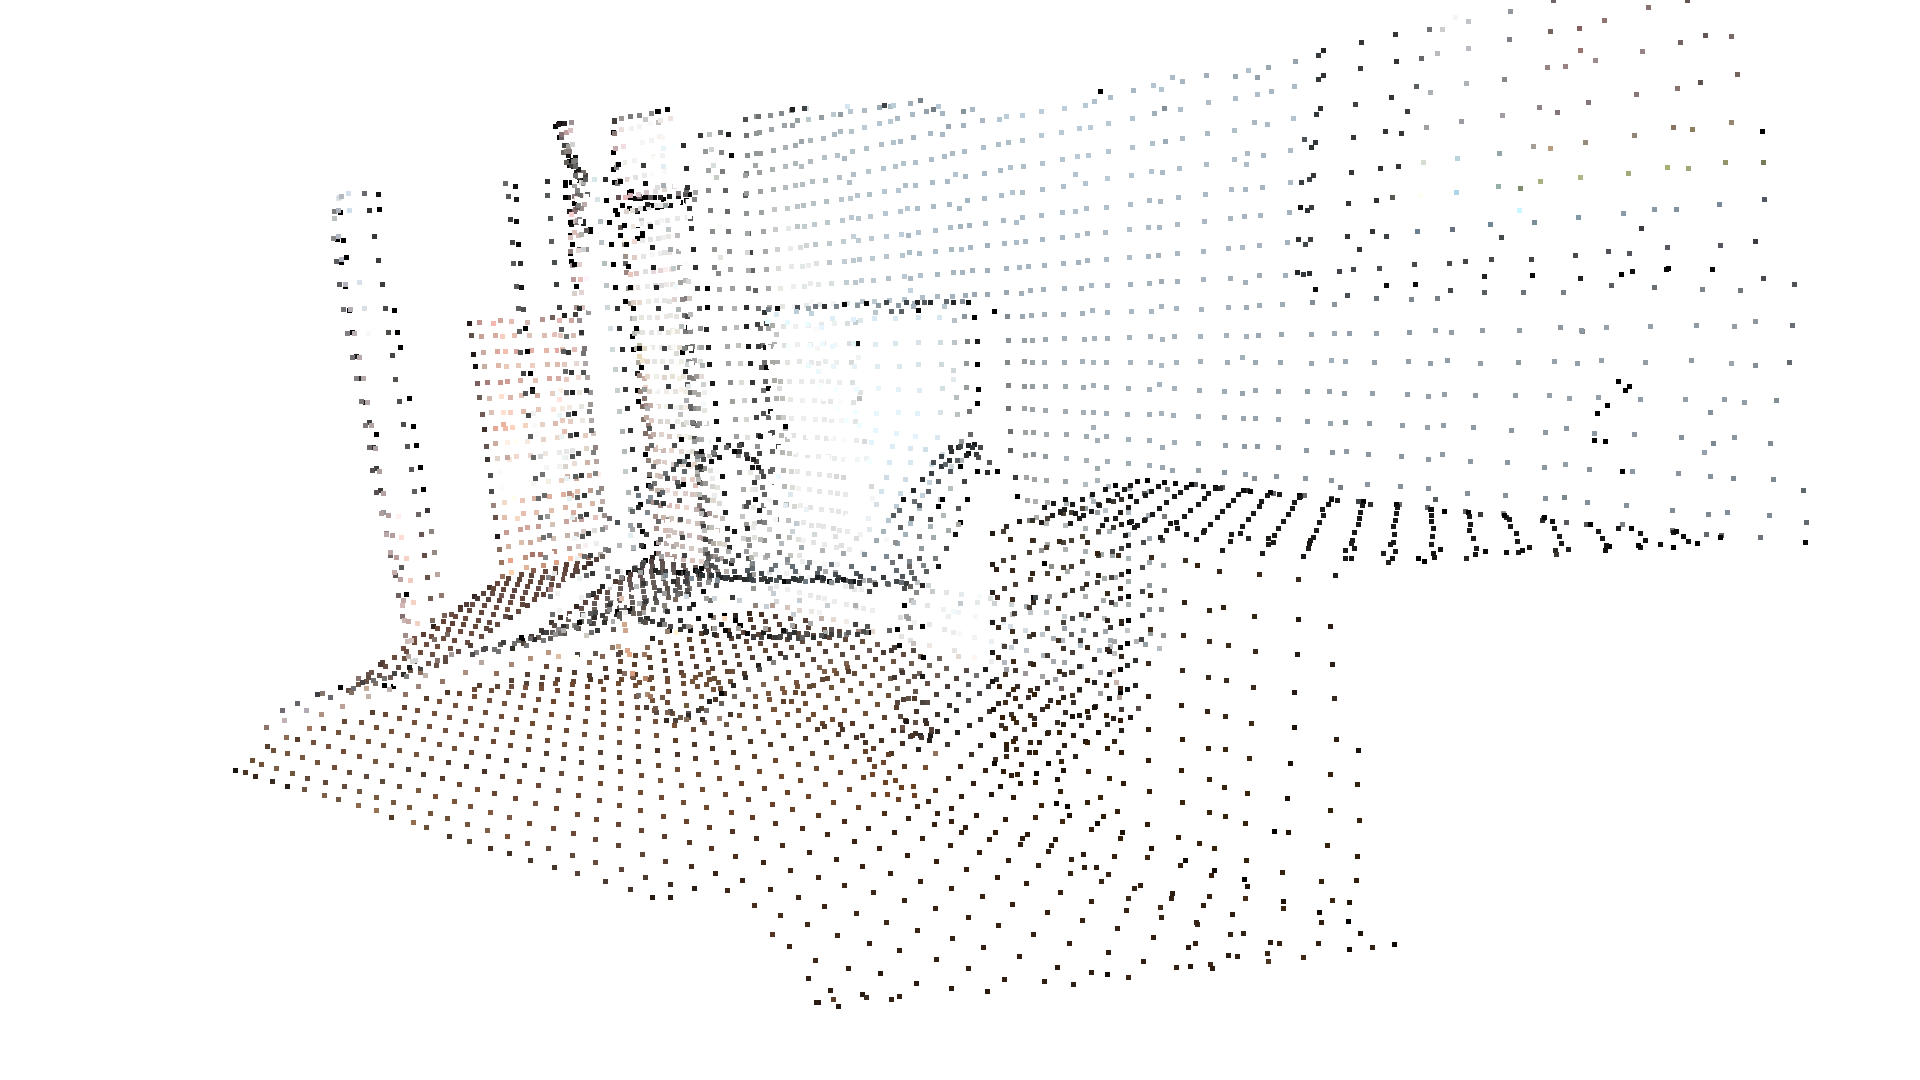
\includegraphics[ width=.5\textwidth ]{PointCloud}
    \caption{Beispiel einer drei-dimensionalen Point-Cloud-Rekonstruktion\label{fig:PointCloud}}\par
\end{figure}

\subsection{Bundle Adjustment}

Der Bundle Adjustment ist ein Optimierungsverfahren, das verwendet wird, um die Kamerapositionen und die 3D-Struktur der Szene zu verfeinern. Dabei werden die Fehler zwischen den projizierten 3D-Punkten und den tatsächlichen 2D-Punkten minimiert, um die bestmögliche Schätzung der Kamerapositionen und der 3D-Struktur zu erhalten. Der Bundle Adjustment ist ein iterativer Prozess, der normalerweise auf der nicht-linearen Optimierung basiert. Es gibt verschiedene Algorithmen zur Bundle Adjustment, wie z. B. die Levenberg-Marquardt-Methode oder die Gauss-Newton-Methode.

\section{Markenbasiertes Tracking}

Beim markenbasierten Tracking werden Feature-Punkte in der echten Welt platziert und anschließend von der Kamera erkannt. In der Abbildung \ref{fig:Marker} ist ein Beispiel für ein markerbasiertes Tracking dargestellt. 

\begin{figure}
    \centering
    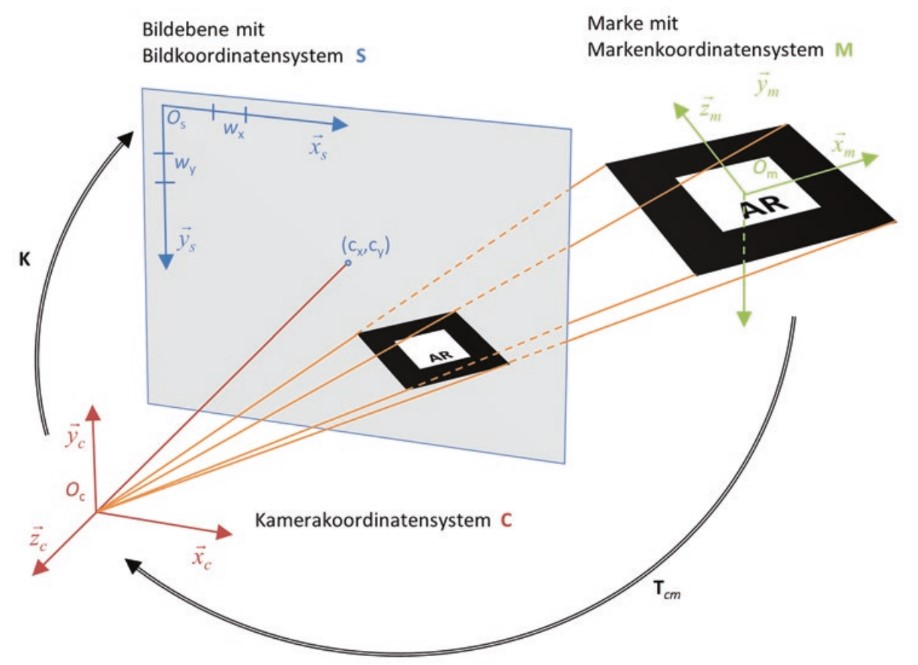
\includegraphics[ width=.5\textwidth ]{Marker}
    \caption{Darstellung eines markenbasiertes Tracking\label{fig:Marker}}\par
\end{figure}

Hier wird mithilfe der intrinsichen und extrinsischen Parameter der Kamera (siehe Kapitel 4.2) die Position und Orientierung des Markers im Raum bestimmt. Dabei nimmt man sich die bekannten Dimensionen des Markers zu Nutze, um eine Transformationsmatrix \(T_cm\) zu berechnen, mithilfe derer man die Koordinaten des Markers im lokalen Koordinatensystem ins Kamerakoordinatensystem transformieren kann. Die Bestimmung der Transformation \(T_cm\) erfolgt funktioniert wie folgt:

Es soll gelten:
\[ v_c = T_cm * v_m \]

Nun gilt für einen Bildpixel \(v_s\) unter Anwendung der intrinsischen Kameraparameter (siehe Kapitel 4.2):
\[ v_s = K * v_c \]

Daraus folgt:
\[ v_s = K * T_cm * v_m \]

Da \(v_s\) und \(v_m\) bekannt sind (die Pixelkoordinaten des Markers und die bekannten Dimensionen des Markers), kann die Transformation \(T_cm\) berechnet werden.

Das markerbasierte Tracking ist besonders robust und präzise, da die Position und Orientierung des Markers bekannt sind. Allerdings ist es auch aufwendiger, da die Marker manuell platziert und kalibriert werden müssen. Es wird häufig in Anwendungen eingesetzt, bei denen die Position des darzustellenden Objekts genau bekannt ist. Auch in der Filmproduktion wird markerbasiertes Tracking oft für Motion-Caputre-Verfahren verwendet.

\section{SLAM}

Simultanous Localization and Mapping (SLAM) entstammt urprünglich aus der Robotik und beschreibt die Fähigkeit eines autonomen Systems, sich in einer unbekannten Umgebung zu lokalisieren und gleichzeitig eine Karte dieser Umgebung zu erstellen. SLAM ist sehr stark mit Structure-from-Motion-Algorithmen verwandt, da beide Techniken die gleichen Prinzipien verwenden, um die Kameraposition und die 3D-Struktur der Szene zu bestimmen. Der grundlegende Unterschied besteht darin, dass SLAM die Priorität auf die Echtzeitverarbeitung und die gleichzeitige Schätzung der Position und Orientierung des Sensors und die dreidimensionale Rekonstruktion der Umgebung legt. 

\section{Scene Understanding}

TODO

\section{Technische Limitationen}

Viele der gängigen Algorithmen zur Feature-Erkennung und -Verfolgung, wie SIFT oder ORB, verlassen sich stark auf die visuelle Qualität der Eingabebilder. In Umgebungen mit schlechten Lichtverhältnissen (z. B. bei schwacher Beleuchtung, direkter Sonneneinstrahlung oder Nachtaufnahmen) wird die Fähigkeit der Algorithmen zur präzisen Merkmalserkennung und -verfolgung beeinträchtigt. Dies kann zu fehlerhaften Schätzungen der Kameraposition oder der 3D-Rekonstruktion führen.

Ein weiteres Problem tritt auf, wenn sich die Umgebung schnell verändert, etwa bei Bewegungen von Objekten, plötzlichen Änderungen der Szene oder in dynamischen Umgebungen. In solchen Fällen können Feature-Punkte in den Bildern verschwinden oder durch neue, nicht korrespondierende Punkte ersetzt werden, was die Stabilität der Berechnungen negativ beeinflusst.

Auch LiDAR-basierte Systeme sind von technischen Einschränkungen betroffen. Zum einen haben LiDAR-Sensoren eine begrenzte Reichweite, die oft auf wenige Meter beschränkt ist, wodurch sie nicht für alle Anwendungen geeignet sind, insbesondere bei großen Distanzen oder in weiten offenen Bereichen.

Zudem sind LiDAR-Sensoren in der Regel teuer und daher nur vereinzelt in Smartphones verbaut. LiDAR-basierte Systeme sind vor allem in spezialisierten Bereichen wie der Automobilindustrie oder der Robotik weit verbreitet, aber in konsumerorientierten Geräten noch eher selten.